\part{Psy}

	\begin{center}
	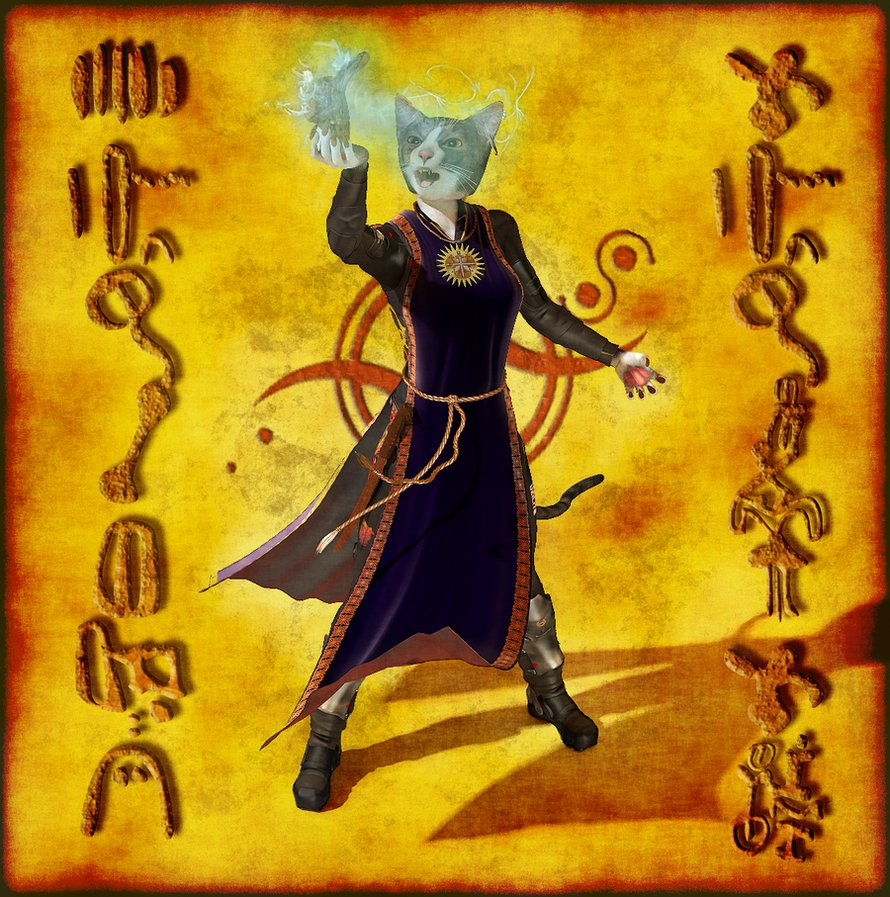
\includegraphics[scale=0.25]{Img/teldrim_psy}
	\end{center}

\chapter{Le psy dans les mondes connus}

\begin{multicols}{2}

Pour la plupart des races, les pouvoirs psy sont un phénomène récent. Pour les Teldrims et les Centauriens, ils font parti intégrante de leur culture.

Les psy Teldrims ont appris à maitriser, via de longs et épuisant rituels, le bois sacré nommé Tellien. Ils peuvent changer sa forme et sa densité. Grâce à cela, le Tellien est devenu la composante principale de leur technologie. La prêtrise a gagné son statut grâce à ce pouvoir. Concernant les Teldrims, on peut donc dire que le pouvoir psy a influencé profondément leur culture.

Les Centauriens ont tous des facultés psy : ils sont liés entre eux télépathiquement. Ils peuvent à tout moment partager des émotions fortes au reste des Centauriens. Les plus doués d'entre eux peuvent même transmettre quelques images, ou quelques mots. C'est ce pouvoir psy qui a fait d'eux ce qu'ils sont aujourd'hui : un peuple extrêmement uni.

Chez les autres peuples, les pouvoirs psy sont un phénomène nouveau. Les psy sont des êtres isolés, des apprentis Sorciers jouant avec le feu en découvrant leurs pouvoirs. Heureusement ils sont peu puissants et les accidents qu'ils entraînent sont peu important. Ils sont toutefois en général très vite surveillés par les autorités qui vérifient qu'ils ne causent pas de dommages majeurs, mais qui contrôlent aussi l'évolution de leurs pouvoirs et leur utilité potentielle.

C'est chez les Snagirs que les psy sont le plus contrôlés. Le Consortium a créé une cellule spéciale chargée de trouver, recruter, et former les psy potentiels. Officiellement cette cellule a uniquement pour but d'éviter les débordements. Toutefois tout le monde suspecte le Consortium d'avoir d'autres vues...

\end{multicols}

\chapter{La marque des Ergios}

\begin{multicols}{2}

Dans l'ensemble, les psy présents dans les mondes connus sont peu puissants. Ils n'utilisent leurs pouvoirs qu'avec difficulté, au prix d'énormement de concentration, voir de rituels complexes. Il y a toutefois des exceptions, des psy capables de tordre la réalité avec la force de leur volonté, capable de le faire avec rapidité. Ces exceptions sont les porteurs de la Marque des Ergios.

La marque des Ergios est un symbole, a priori d'origine Ergios, présent sur le haut du corps des marqués. Ce symbole occupe un cercle d'environ 10 cm de diamètre. En temps normal, la marque est totalement invisible. Elle apparaît uniquement lorsque son porteur se concentre pour utiliser un pouvoir psychique. Durant toute l'utilisation, elle s'illumine. Une fois que le psy arrête de se concentrer, elle s'estompe peu à peu jusqu'à disparaître totalement.

Les marqués sont des psy extrêmement puissants. Les premiers marqués sont apparus il y a très peu de temps, lors de l'attaque de la capitale par les Eskadors. En plus d'utiliser les pouvoirs psy connus avec une aisance surprenante, certains développent des pouvoirs totalement inédits.

Les marqués intriguent, inquiètent. Certains voient le potentiel qu'ils représentent et veulent les utiliser, certains voient en eux un danger et aimeraient les réduire au silence. Tous se demandent ce que représentent cette étrange marque, et d'où elle vient...

\end{multicols}

\note{Le cas de l'Impératrice Eternelle}{

Les Vélïos ont déjà vu ou entendu parler de ce type de marque. Leurs rangs comptent un marqué depuis des siècles : l'impératrice éternelle. La marque de celle-ci s'étend toutefois sur l'intégralité de son corps. Peu de Vélïos ont directement vu l'impératrice éternelle, mais ces marques font partie de leurs légendes...

}

\chapter{Description des pouvoirs}

\begin{multicols*}{2}

Les pouvoirs de psy, et tout particulièrement ceux des "marqués" sont très peu connus. Les pouvoirs ci-dessous correspondent aux pouvoirs qui ont déjà pu être constatés et référencés. Cette liste n'est donc pas forcément exhaustive.

\section{Télépathie}

Ce pouvoir est l'évolution du pouvoir des Centauriens. Un "marqué" ayant développé le pouvoir de télépathie sera lié avec les Centauriens et pourra partager des informations par ce lien si particulier. Contrairement aux centauriens de base, il pourra passer plus que de simple émotions, il pourra transmettre des phrases, des images. Il sera même capable de choisir à qui son message est destiné.

Selon la rumeur, les marqués seraient aussi capables d'étendre leur télépathie, dans une moindre mesure, aux non-centauriens. On raconte qu'ils pourraient aussi lire dans nos pensées...

Il est à noter que les Centauriens voient très mal l'existence de personnes partageant leur lien sans faire partie de leur peuple.

\section{Telien}

Ce pouvoir permet de contrôler par la pensée le bois sacré des Teldrims : le Tellien. Le psy serait capable de modifier sa forme, sa densité, et même de le rendre conducteur. Contrairement aux prêtres Teldrim, un marqué pourrait faire tout cela en quelques secondes à peine.

Pour le peuple Teldrim, ce pouvoir est reservé à leur prêtrise. Un personnage non-teldrim (ou même teldrim esclave ! ) utilisant le Telien risquerait de provoquer le courroux de ce peuple très croyant.

\section{Esprit de la machine}

Ce pouvoir permet de communiquer avec les machines par la force de la pensée, de les influencer, et de leur commander. Ce pouvoir concerne aussi bien l'informatique, les machines électroniques, que les machines mécaniques.

\section{Contrôle du corps}

Ce pouvoir permet au psy de contrôler son propre corps pour le rendre plus résistant, plus fort, plus rapide, ... Le psy pourrait aussi se placer dans un état de stase, proche de la mort, ou même augmenter ses différents sens.

Selon les récits rapportés par des Vélïos, l'impératrice éternelle semble dotée de ce pouvoir. Les légendes Vélïos sont remplies d'exploits de l'impératrice qui aurait été capable de régénerer ses blessures, ou même de faire repousser un de ses membres. De plus selon la légende, l'impératrice éternelle est la même depuis de longs siècles.

\section{Contrôle de la gravité}

Ce pouvoir permet de contrôler la gravité pour l'amplifier, ou au contraire la diminuer voir l'éliminer totalement. Le psy peut choisir la zone sur laquelle s'applique son pouvoir. Un psy utilisant ce pouvoir pourrait donc se faire "léviter" en supprimant sur lui l'effet de la gravité, rendre particulièrement lourd un de ses opposants, ou même faire décoller un véhicule par la seule force de sa volonté.

\section{Contrôle de l'énergie}

Ce pouvoir permet de contrôler l'énergie sous toutes ses formes. Un Psy utilisant ce pouvoir pourrait créer des vagues d'énergie, recharger ou vider une batterie ou même un réacteur, créer une surcharge électrique dans un appareil, ...

\section{Porte vers le second espace}

Ce pouvoir permet à son possesseur de créer un trou de ver l'emmenant dans le second espace. L'utilisateur peut ensuite quitter cette dimension quand il le désire pour revenir dans le monde normal, effectuant une sorte de téléportation. 

Toutefois le second espace est un endroit étrange, n'offrant que très peu de repères au psy pour déterminer sa direction et la distance à parcourir. De plus les légendes racontent qu'il y a des bêtes qui rôdent dans ce monde, des bêtes dangereuses qui pourraient bien s'en prendre au psy.

Le psy est capable d'emmener des objets ou d'autres personnes avec lui. Bien sûr plus le nombre et/ou la taille des choses emportées avec lui sont grands, plus difficile est la création du trou de ver.

\section{Forme-esprit}

Grâce à ce pouvoir, l'utilisateur détache son esprit de son corps. L'esprit devient alors une forme, ressemblant au corps du personnage, mais totalement intangible. Ce corps est à la fois visible dans le monde réel et dans le second espace. Sous sa forme-esprit, le psy ne voit plus que ce qui est vivant (dans un monde ou dans l'autre). La façon dont il perçoit les choses dépend aussi de leur sensibilité psy : un non-psy apparait très terne, un psy brille légèrement, un marqué brille de mille feux tel un phare.

\end{multicols*}
